% chapter_11_DIGI.tex -- chapter 11 of the JitJet book: the digitisation, with and without pileup.
% Every number comes from test/11_DIGI/out/ (ledger_11_DIGI.txt, digiAnalyzer_{signal,pileup,mixed}_11_DIGI.log,
% thresholds_11_DIGI.txt, trigprim_11_DIGI.txt, examples_11_DIGI.txt, the PNG pages), from test/10_SIM/out/
% (simHits_signal_10_SIM.log, step3_MIX_10_SIM.log), from the FWLite extras and the conddb dumps listed in
% doc/chapter/chapter_11_DIGI.md, section 4.
% B3 is split into one subsection per digitiser (the teaching layout of chapters 09-11): what it does, the
% parameters, the numbers of the event, a figure.

\chapter{11 -- DIGI: the hits become electronics signals and the pileup is mixed in}
\label{ch:11_DIGI}

\section{What this chapter is about}

Geant4 left the event as energy deposits: \code{PSimHit}s in the silicon sensors and muon chambers, \code{PCaloHit}s
in the calorimeter cells, each with a time and, through the \code{SimTrack}, a particle. No detector delivers that. A
detector delivers what its \emph{front-end electronics} makes of the deposits: a silicon sensor collects the charge
that a particle freed, an amplifier turns it into a voltage pulse a few tens of nanoseconds long, an analogue-to-digital
converter (ADC) samples the pulse every 25\,ns, noise is added on the way, and only the channels above a threshold are
kept. The \code{DIGI} step (\code{cmsDriver.py -s DIGI:pdigi\_valid}) simulates exactly this, one \emph{digitiser} per
subdetector. What comes out is a \emph{digi}: a channel number and a few integers, what the detector would have sent
to the data acquisition. Every later stage of the journey, the trigger as much as the reconstruction, sees only digis.

It is also the step where the pileup enters. Before the digitisers run, the \code{MixingModule} of
chapter~\ref{ch:10_SIM} overlays on the hits of the signal those of the other collisions of the bunch crossing and of
the neighbouring crossings, each shifted in time by its distance to ours. The electronics cannot tell a signal hit from
a pileup hit: the charges of a channel are added before anything else happens. The simulation keeps a record all the
same: in the tracker and in the muon chambers a \code{DigiSimLink} says, channel by channel, which simulated particle
put charge there; in the calorimeters the signal and the pileup fall into the same data frame and nothing in it says
who deposited what. Figure~\ref{fig:11_chain} is the chain every digitiser follows.

\begin{figure}[!htb]
\centering
\begin{tikzpicture}[x=1cm, y=1cm, font=\footnotesize, >={Stealth[length=2mm]},
  box/.style={draw, rounded corners=2pt, minimum height=12mm, text width=2.25cm, align=center, inner sep=2pt},
  inp/.style={box, fill=black!6, text width=3.3cm, minimum height=6.5mm},
  mix/.style={box, fill=orange!15, text width=3.6cm, minimum height=26mm},
  st/.style={box, fill=blue!8}, outb/.style={box, fill=green!12}, tp/.style={box, fill=red!10, text width=3.3cm, minimum height=9mm}]
\node[inp] (s)  at (1.65,3.15) {the signal, bx 0};
\node[inp] (m1) at (1.65,2.35) {71 collisions, bx $-1$};
\node[inp] (z)  at (1.65,1.55) {68 collisions, bx 0};
\node[inp] (p1) at (1.65,0.75) {54 collisions, bx $+1$};
\node[mix] (mix) at (6.2,1.95) {\code{MixingModule} \code{mix}\\[1pt] replays the draw of chapter~\ref{ch:10_SIM} (playback)\\[1pt] one \code{CrossingFrame} per hit collection};
\foreach \n in {s,m1,z,p1} \draw[->] (\n.east) -- (mix.west|-\n.east);
\node[text width=6.4cm, align=left, font=\scriptsize] at (11.85,1.95) {The pixel, strip, ECAL and HCAL digitisers run \emph{inside}
\code{mix} (\code{process.mix.digitizers}: \code{pixel}, \code{strip}, \code{ecal}, \code{hcal}), first on the signal hits, then on the
pileup hits of each bunch crossing, before the \code{CrossingFrame}s are thrown away. The muon digitisers and the
calorimeter zero suppression are modules of their own, after \code{mix}.};
\node[st] (c1) at (0.0,-0.75) {SimHit\\{\scriptsize energy, time, position}};
\node[st] (c2) at (2.65,-0.75) {charge or light\\{\scriptsize $e$--$h$ pairs, photo\-electrons}};
\node[st] (c3) at (5.3,-0.75) {pulse shaping\\{\scriptsize APV25, MGPA, QIE}};
\node[st] (c4) at (7.95,-0.75) {sampling\\{\scriptsize one value per 25\,ns}};
\node[st] (c5) at (10.6,-0.75) {$+$ noise, pedestal, gain, ADC};
\node[outb] (c6) at (13.25,-0.75) {thresholds, zero suppression, selective readout $\rightarrow$ \textbf{digi}};
\foreach \a/\b in {c1/c2,c2/c3,c3/c4,c4/c5,c5/c6} \draw[->] (\a) -- (\b);
\draw[->] (mix.south) -- ++(0,-0.35) -| (c1.north);
\node[tp] (tp) at (10.6,-2.35) {calorimeter trigger primitives (section~\ref{sec:11_tp})};
\draw[->] (c5.south) -- (tp.north);
\draw[->] (tp.east) -| (c6.south);
\node[font=\scriptsize, align=center] at (13.6,-2.85) {drive the ECAL\\selective readout};
\draw[->] (tp.west) -- ++(-1.3,0) node[above, pos=0.5, font=\scriptsize] {to ch.~\ref{ch:12_L1T}};
\node[text width=6.6cm, align=left, font=\tiny] at (3.15,-2.55) {\ttfamily simSiPixelDigis, simSiStripDigis:ZeroSuppressed,\\
simEcalUnsuppressedDigis $\rightarrow$ simEcalDigis, simEcalPreshowerDigis,\\
simHcalUnsuppressedDigis $\rightarrow$ simHcalDigis,\\ simMuonDTDigis, simMuonCSCDigis, simMuonRPCDigis, simMuonGEMDigis};
\end{tikzpicture}
\caption{The chain of the \code{DIGI} step. Top: the hits of the signal and of the 193 pileup collisions of chapter~\ref{ch:10_SIM}
are put side by side, each collision shifted in time by $25\ns$ per bunch crossing (bx). Bottom: what every digitiser
does to the hits of one channel, and the modules that write the digis (bottom left). The calorimeters make, from
their unsuppressed frames, a coarse copy for the Level-1 trigger, which in the ECAL also decides which frames are
written.}
\label{fig:11_chain}
\end{figure}

\begin{table}[!htb]
\centering\small\setlength{\tabcolsep}{3.5pt}
\caption{The digitisers at a glance: what the electronics does, and what goes in and comes out for the signal alone
and for the signal with its bunch crossing (\code{ledger\_11\_DIGI.txt}; the HCAL frames from the FWLite extras of the
companion). Each row is one subsection of section~\ref{sec:11_numbers}.}
\label{tab:11_glance}
\begin{tabular}{@{}l>{\raggedright\arraybackslash}p{5.0cm}>{\raggedright\arraybackslash}p{3.0cm}rr@{}}
\toprule
 & what the electronics does & signal: in & signal: out & with pileup: out \\
\midrule
mixing & overlays 193 collisions of bx $-1$, 0, $+1$, times shifted by $\mp25\ns$ & 10\,272 tracker hits & -- & 448\,315 tracker hits \\
pixels & charge above 1600--2000\,$e$ in a $100\times150\,\mu$m$^2$ pixel, an 8-bit ADC, a $\pm12.5\ns$ window & 1902 \code{PSimHit}s & 4800 digis & 77\,980 \\
strips & APV25 pulse in deconvolution mode, zero suppression at 5 (2) times the noise & 8370 \code{PSimHit}s & 31\,602 digis & 436\,901 \\
ECAL, ES & photoelectrons, 10 samples of 25\,ns, selective readout; ES 3 samples & 5521 + 6214 + 1069 cells & 156 + 384 + 981 & 964 + 2520 + 15\,972 \\
HCAL & SiPM or PMT, QIE charge code, 10 (HF: 3) slices, zero suppression & 821 HB/HE, 1 HO, 531 HF cells & 4459 + 0 + 3456 & 6545 + 2 + 3456 \\
muon & drift times, strip samples, bunch crossings & no hit & 8 (RPC noise) & 2016 \\
\midrule
all & & & 44\,172 & 544\,407 \\
\bottomrule
\end{tabular}
\end{table}

The chapter digitises three samples with the same configuration (\path{test/11_DIGI/run_11_DIGI.sh}): (11a) the signal
alone, no mixing; (11b) one library collision alone, library event 72, the first in-time collision of our bunch
crossing; and (11a+11b) the production case, the signal with its 71, 68 and 54 collisions in bunch crossings $-1$, 0
and $+1$. The sample (11b) exists only in this book: in the production the collisions are never digitised one by one.
Run~3 and Phase-2 use \emph{premixing}: a first job mixes and digitises the whole pileup of a bunch crossing into a
library of premixed events (\code{premix\_stage1}), a second job digitises the signal alone and adds one premixed
event to it digi by digi (\code{PreMixingModule}, \path{Configuration/StandardSequences/python/DataMixerPreMix_cff.py}).
The classical mixing of this chapter does the same in one job and keeps every pileup hit in memory, which is what
lets the analyzer tell the origin of every digi.

\emph{How the chapter is organised.} Section~\ref{sec:11_numbers} has one subsection per row of
table~\ref{tab:11_glance}: the mixing and the time windows, then the pixels, the strips, the ECAL, the HCAL and the
muon chambers. Each says, like a step of chapter~\ref{ch:12_L1T}, what the electronics does, which parameters decide
it and where they are set, and what it made of our event, with one data frame or one channel followed by hand. A
subsection then puts the three samples side by side and one says what the 2025 conditions changed. The section
``Made here for the next stage'' explains the calorimeter trigger primitives that this job makes for the Level-1
trigger of chapter~\ref{ch:12_L1T}.

\section{From the previous chapter}

Three files of chapter~\ref{ch:10_SIM} enter (Rule E). The signal, \path{test/10_SIM/out/step2_SIM_signal_10_SIM.root},
is the full Geant4 event: 1926 \code{SimTrack}s from 571 primaries, $10\,272$ tracker \code{PSimHit}s (PXB 929, PXF 973,
TIB 1182, TID 975, TOB 1022, TEC 5191, $2.33\GeV$ of energy loss) and $26\,793$ \code{PCaloHit}s in $14\,157$ cells
(EB 5521 cells with $68.0\GeV$, EE 6214 with $293.7\GeV$, ES 1069, HB 173, HE 648, HO 1, HF 531 cells with 1849
photoelectrons of the shower library), no muon-chamber hit. The library,
\path{step2_SIM_pileup_10_SIM.root}, holds the 250 minimum-bias collisions through the same Geant4; library event 72
has 164 primaries, 2097 tracker hits, 11 CSC hits, 1217 EB cells with $9.4\GeV$, 1948 EE cells with $43.5\GeV$, 223
ES, 21 HB, 101 HE and 119 HF cells. The third file, \path{step3_MIX_10_SIM.root}, is the signal again with one new
product: the \code{CrossingFramePlaybackInfoNew} that the chapter-10 mixing job wrote, the list of which library
events it drew into which bunch crossing. That mixing put $448\,315$ tracker \code{PSimHit}s in front of the
digitisers: $10\,272$ of the signal, $146\,028$ of the 68 in-time collisions, $139\,551$ of the 71 early ones and
$152\,464$ of the 54 late ones.\footnote{Signal hits from \path{test/10_SIM/out/simHits_signal_10_SIM.log}, the
bunch crossing from \path{step3_MIX_10_SIM.log}; library event 72, the zero suppression and the truth counts from
FWLite (companion, section~4); every digi count from \path{test/11_DIGI/out/ledger_11_DIGI.txt}; the data frames
followed by hand and the charges from \path{examples_11_DIGI.txt} (\path{test/11_DIGI/digiExamples_11_DIGI.py}).}

The job runs with the 2025 settings of the release, as chapters~\ref{ch:08_PU}--\ref{ch:10_SIM}; unlike there, the
year changes the result here, because the digitisers read conditions of the global tag that differ in 2025 (the
python thresholds are those of 2024). Section~\ref{sec:11_year} says what changed.

\begin{plainwords}[What a digi is]
A pixel digi is a pixel address and an 8-bit ADC count; a strip digi the same for a strip, kept only if it passed the
zero suppression of the front-end driver; an ECAL digi is a \emph{data frame}, the ten 40-MHz samples of the pulse of
one crystal with the gain of each sample; an HCAL digi is the QIE frame, 10 (HB, HE) or 3 (HF) time slices of the
charge; a DT digi is a wire and a drift time, a CSC digi a strip with 8 samples or a wire group with a time, an RPC
or GEM digi a strip and a bunch crossing. The digitisers are configured in the python of the \code{DIGI} process
(\code{process.mix.digitizers} for the tracker and the calorimeters, the modules \code{simMuon*Digis} for the
chambers); \path{test/11_DIGI/out/thresholds_11_DIGI.txt} lists every threshold, noise and window the job used.
\end{plainwords}

Nothing of the SIM content changes: the \code{DIGI} process copies the generator record, the \code{SimTrack}s and
the signal hits unchanged and adds its products under the process name \code{DIGI}: one digi collection per
subdetector (\code{simSiPixelDigis}, \code{simSiStripDigis}, \code{simEcalDigis}, \code{simHcalDigis},
\code{simMuon*Digis}, \ldots), the \code{DigiSimLink}s, the trigger primitives, the \code{TrackingParticle}s of
\code{mix:MergedTrackTruth} (999 for the signal, $45\,282$ in the mixed event, of which $14\,729$ in-time and
$29\,554$ out-of-time pileup) and the \code{PileupSummaryInfo} with the number of collisions per bunch crossing. The
pileup \code{SimTrack}s and hits themselves are not written; the \code{CrossingFrame}s live only inside the job.

\section{The numbers of the event}
\label{sec:11_numbers}

Table~\ref{tab:11_cuts} is the part of \path{thresholds_11_DIGI.txt} that decides what becomes a digi; the
subsections below take it row by row. Two things are worth seeing at once. First, several thresholds are not numbers
in the configuration but database payloads of the global tag \code{150X\_mcRun3\_2025\_realistic\_v1}: the strip
zero-suppression thresholds, the ECAL selective-readout settings (\code{configFromCondDB = True}), the preshower
threshold and the HCAL zero-suppression levels (\code{useConfigZSvalues = 0}: the \code{HBlevel = 8}, \code{HElevel =
9}, \code{HOlevel = 24} of the python are not used). Second, the time windows differ by an order of magnitude between
subdetectors, and this is what decides how much of the out-of-time pileup survives.

\begin{table}[htb]
\centering\footnotesize\setlength{\tabcolsep}{4pt}
\caption{The cuts of the digitisers of the mixed configuration (\code{test/11\_DIGI/out/thresholds\_11\_DIGI.txt}, the
parameter sets of \code{process.mix.digitizers} and of the modules after the mixing; the payloads from \code{conddb
dump}, companion section~4). ``DB'' means the value is a payload of the global tag, not a number in the python.}
\label{tab:11_cuts}
\begin{tabular}{p{1.4cm}p{14.2cm}}
\toprule
digitiser & what decides whether a channel becomes a digi \\
\midrule
pixel & charge above \code{ThresholdInElectrons} $=1600$\,e (BPix layer 1: 2000\,e), smeared by 245\,e (BPix) / 210\,e
(FPix); noise 175\,e per pixel plus 350\,e readout noise, noisy pixels added; ADC from a fixed non-linear response
(\code{BPix\_SignalResponse\_p0..p3}), 8 bits; time window \code{TofLowerCut/TofUpperCut} $=-12.5/+12.5\ns$; Lorentz
angle, dead modules and bad FED channels from DB; inefficiency on \\
strip & APV in deconvolution mode, hits within \code{TOFCutForDeconvolution} $=50\ns$, weighted by the APV pulse
(\path{APVShapeDeco_320.txt}); per-strip pedestals and noise from DB, common-mode noise RMS 5.92 / 3.08 / 1.08 / 2.44
ADC (TIB / TID / TOB / TEC); 247\,e per ADC count; FED zero suppression \code{FedAlgorithm = 4}: a strip above 5 times
its noise, or above 2 times with a neighbour above 2 times (DB, \code{SiStripThreshold\_Ideal\_31X\_v2}) \\
ECAL & 2250 (EB) / 1800 (EE) photoelectrons per GeV, laser correction from DB, pulse shape from DB, 10 samples, peak
in sample 6, correlated noise (the \code{CorrNoiseMatrix} vectors), constant term 0.3\,\%; selective readout
(\code{simEcalDigis}) from DB, driven by the trigger primitives: full readout of the trigger towers / supercrystals
flagged high interest, zero suppression elsewhere ($0.3325\GeV$ EB, $0.36\GeV$ EE); ES: 3 samples, threshold of 6 ADC
counts on sample 2 (DB, \code{ESThresholds\_LG\_V03\_mc}) \\
HCAL & HB / HE: photoelectrons per GeV from the sampling factors 125 (HB) and 186--211 (HE) and the gain and SiPM
parameters of DB, SiPM and time smearing, 10 time slices with the sample of interest at 6, TDC threshold 18.7; HF:
6 photoelectrons per shower-library unit, sampling factor 0.37, 3 time slices; zero suppression (\code{simHcalDigis})
on the sample of interest (\code{use1ts}) with levels from DB, none for HF; a frame for every channel
(\code{doEmpty = True}) \\
muon & DT: drift time smeared by 2.4\,ns, dead time 150\,ns, links within 10\,ns; CSC: strip pedestals, gains and noise
from DB (\code{stripConditions = Database}), 8 SCA samples of 50\,ns, strips integrated from $-250$ to $+500\ns$,
read in boards of 16 strips; RPC: efficiency 0.95, gate 25\,ns, noise and background on; GEM: efficiency 0.98,
intrinsic noise off, window bx $-5$ to $+3$ \\
\bottomrule
\end{tabular}
\end{table}

\subsection{The mixing, and the time windows of the digitisers}
\label{sec:11_mix}

\textbf{What it does.} The \code{MixingModule} reads, for every bunch crossing of its window, the requested number of
library collisions and gives each of their hits two labels: the bunch crossing and the number of the collision in it,
packed into an \code{EncodedEventId}. It also shifts the time of every hit by $25\ns$ per bunch crossing
(\path{SimGeneral/MixingModule/plugins/Adjuster.cc}: \code{timeOffset = bcr * bunchSpace}): a hit of
bunch crossing $-1$ arrives $25\ns$ before ours, one of $+1$ $25\ns$ after. The hits of all collisions and of the
signal are then put in one \code{CrossingFrame} per collection, and the digitisers inside the module run on it. Nothing
in the digitisers knows about collisions: they see charges arriving at times, and the time is what will separate the
crossings, or fail to.

\textbf{The parameters.} \code{AVE\_60\_BX\_25ns} with \code{N = 60}, \code{B = (-1, 1)}: a Poisson draw of mean 60
collisions in each of three crossings $25\ns$ apart, the library read in sequence (\code{input.sequential = True}) and,
for this book, \code{playback = True} (box below).

\begin{plainwords}[Why the DIGI job replays the chapter-10 draw]
The \code{MixingModule} draws the number of collisions per bunch crossing from a Poisson distribution of mean 60
(seed 12345 of the module \code{mix}) and reads the library in sequence. Chapter~\ref{ch:10_SIM}
drew 71, 68 and 54. The same module with the same seed in this chapter would \emph{not}: in
\code{BMixingModule::produce} (\path{Mixing/Base/src/BMixingModule.cc}) the order is \code{initializeEvent},
\code{addSignals}, then \code{doPileUp}, and \code{addSignals} runs the digitisers on the signal, which consume random
numbers from the same engine (noise, photostatistics, threshold smearing) before \code{PileUp::CalculatePileup}
(\path{Mixing/Base/src/PileUp.cc}, called from \path{SimGeneral/MixingModule/plugins/MixingModule.cc}) draws the
number of collisions. In chapter~\ref{ch:10_SIM} no digitiser ran, so the draw came first; here a fresh draw gave
65, 67 and 56 when it was tried. The script therefore sets \code{process.mix.playback = True}: the module reads the
\code{CrossingFramePlaybackInfoNew} of \path{step3_MIX_10_SIM.root} and mixes exactly library events 1--71, 72--139
and 140--193; the \code{PileupSummaryInfo} then reports 71, 68 and 54 as the ``true'' number of interactions, not 60.
\end{plainwords}

\textbf{The time windows.} Each digitiser looks at a different stretch of time around our crossing, and
figure~\ref{fig:11_windows} draws them on one axis. The pixels accept a hit only if it arrives within $\pm12.5\ns$ of
the time a particle travelling at the speed of light from the centre of the detector would need
(\code{TofLowerCut/TofUpperCut}): one crossing, nothing else. The strips accept $\pm50\ns$, but weight the charge with
the APV pulse, which is non-zero only from $28\ns$ before to $30\ns$ after its peak. The calorimeters write ten
samples of $25\ns$, from five samples before the in-time peak to four after it, and their pulses last longer than
that. The muon chambers are slower still: a DT wire sees electrons drift for hundreds of nanoseconds, a CSC strip
integrates from $-250$ to $+500\ns$. The mixing of this book offers three crossings; the production profile of 2025
mixes from $-12$ to $+3$ (chapter~\ref{ch:10_SIM}), because the slow detectors remember that far back.

\begin{figure}[!htb]
\centering
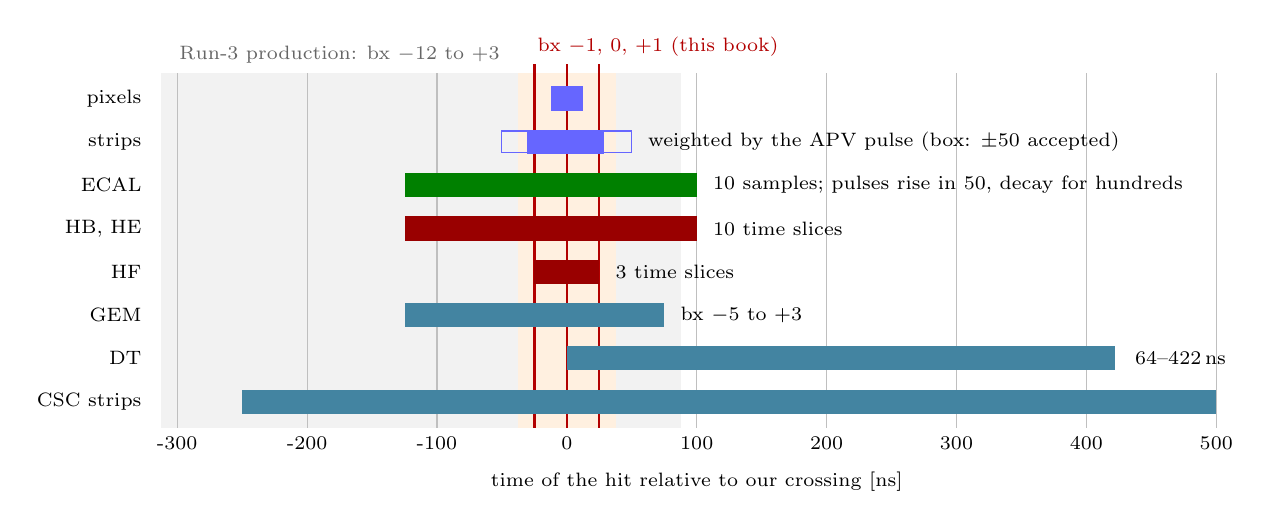
\begin{tikzpicture}[x=0.0165cm, y=0.55cm, font=\scriptsize]
\fill[orange!12] (-37.5,0.4) rectangle (37.5,8.6);
\fill[black!5] (-312.5,0.4) rectangle (-37.5,8.6); \fill[black!5] (37.5,0.4) rectangle (87.5,8.6);
\foreach \t in {-300,-200,-100,0,100,200,300,400,500} { \draw[black!25] (\t,0.4) -- (\t,8.6); \node[below] at (\t,0.4) {\t}; }
\foreach \t in {-25,0,25} \draw[red!70!black, thick] (\t,0.4) -- (\t,8.8);
\node[above right, red!70!black] at (-30,8.75) {bx $-1$, 0, $+1$ (this book)};
\node[black!60, above] at (-175,8.6) {Run-3 production: bx $-12$ to $+3$};
\node[below] at (100,-0.4) {time of the hit relative to our crossing [ns]};
\foreach \y/\lab/\a/\b/\c in {8/pixels/-12.5/12.5/blue!60, 7/strips/-30.5/28.4/blue!60,
  6/ECAL/-125/100/green!50!black, 5/{HB, HE}/-125/100/red!60!black, 4/HF/-25/25/red!60!black,
  3/GEM/-125/75/cyan!60!black, 2/DT/0/422/cyan!60!black, 1/CSC strips/-250/500/cyan!60!black}
  { \node[left] at (-320,\y) {\lab}; \fill[\c] (\a,\y-0.28) rectangle (\b,\y+0.28); }
\draw[blue!60] (-50,6.75) rectangle (50,7.25);
\node[right] at (55,7) {weighted by the APV pulse (box: $\pm50\ns$ accepted)};
\node[right] at (105,6) {10 samples; pulses rise in $50\ns$, decay for hundreds};
\node[right] at (105,5) {10 time slices};
\node[right] at (30,4) {3 time slices};
\node[right] at (80,3) {bx $-5$ to $+3$};
\node[right] at (430,2) {64--422\,ns};
\end{tikzpicture}
\caption{The time windows of the digitisers (schematic; the limits are the parameters of \code{thresholds\_11\_DIGI.txt}
and of the muon \code{cfi} files, the pulse limits those of figures~\ref{fig:11_si} and~\ref{fig:11_frames}). Red lines:
the three bunch crossings mixed in this book (orange band); grey: the out-of-time window of the 2025 production
profile, $-12$ to $+3$. The DT bar spans the 12 DT digis of the event, 64 to $422\ns$ after the fixed offset of the
synchronisation.}
\label{fig:11_windows}
\end{figure}

\textbf{The numbers of the event.} The \code{CrossingFrame}s hold $448\,315$ tracker hits: $10\,272$ of the signal,
$146\,028$ in time, $139\,551$ early and $152\,464$ late. Two thirds of what the tracker digitisers receive is out of
time, and the windows decide what becomes of it: the pixels make $77\,980$ digis of their $87\,653$ hits (0.9 per hit,
against 2.5 for the signal alone), the strips $436\,901$ of their $360\,662$ (1.2 per hit). The truth survives the
mixing: $45\,282$ \code{TrackingParticle}s, 999 of the signal, $14\,729$ of the in-time and $29\,554$ of the
out-of-time collisions.

\FloatBarrier
\subsection{The pixels}
\label{sec:11_pixel}

\textbf{What it does.} A pixel module is a sensor of silicon, 285\,$\mu$m thick in the simulated geometry
(\path{Geometry/TrackerCommonData/data/PhaseI/pixbarladder.xml}, \code{SensorThick}), divided into pixels of
$100\times150\,\mu$m$^2$ and bump-bonded to readout chips (ROCs) of $80\times52$ pixels
(\path{trackerStructureTopology.xml}). A charged particle frees one electron--hole pair per $3.61$\,eV it loses
(\code{GeVperElectron} of the pixel digitiser, \path{SiPixelDigitizerAlgorithm.cc}). The digitiser cuts
the path of the \code{PSimHit} into segments, draws the energy loss of each with Landau fluctuations, and drifts the
electrons to the readout side of the sensor. On the way two things spread them: diffusion ($3.7\,\mu$m per
$300\,\mu$m of drift, \code{Sigma0}), and the magnetic field. In the $3.8$\,T field the electrons do not drift straight
along the electric field but at the \emph{Lorentz angle} to it, so that the charge made at the far side of the sensor
lands tens of micrometres sideways. The charge collected by each pixel is compared with a threshold, and a pixel above it
becomes a digi with an 8-bit ADC count.

\textbf{The parameters.} The threshold is 1600 electrons (2000 in the first barrel layer), smeared from pixel to pixel
by 245 (210 in the disks); the noise is 175 electrons per pixel. The ADC is not a straight line: the digitiser
converts the charge to the calibration unit of the chip (\code{ElectronsPerVcal = 47}, 50 in layer~1) and applies the
response $148+203\tanh(0.00171\,v-0.711)$ of the \code{SignalResponse} parameters, which saturates at 255
(figure~\ref{fig:11_si}, left). The Lorentz angle comes from the payload
\code{SiPixelLorentzAngleSim\_phase1\_EoR3\_HV800\_Tr2000}: $\tan\theta_L$ per tesla 0.0358 in layer~1, 0.0709 in
layers 3 and 4.

\begin{plainwords}[A worked example: one particle through one pixel module]
The signal has 592 barrel-pixel hits that cross the full 285\,$\mu$m. Their charge per micrometre of path has a median
of 84 electrons (\code{examples\_11\_DIGI.txt}), so a particle crossing at right angles frees about $84\times285=
24\,000$ electrons: \emph{fifteen times} the threshold of 1600, \emph{140 times} the noise of a pixel. That margin is
why the pixels are clean: not one of the 4800 pixel digis of the signal is noise. In layer~1 the Lorentz angle moves the
charge of the far side by $0.0358\times3.8\times285 = 39\,\mu$m, two fifths of a pixel, in layers 3 and 4 by
$77\,\mu$m: the charge is shared by neighbouring pixels, and the reconstruction will use the sharing to measure the
position better than the pitch. Shared among 2.5 pixels, $24\,000$ electrons give some 9600 per pixel, ADC 78 on the
curve; the median pixel digi of the signal has ADC 69.
\end{plainwords}

\textbf{The numbers of the event.} The 1902 pixel hits of the signal become 4800 digis, 2.5 per hit, all linked to a
signal particle (PXB 3011, PXF 1789). Their ADC counts have a median of 69 (a quarter below 46, a quarter above 105),
and 170 are at full scale, 255: the response saturates at $35\,600$ electrons, which a slow or grazing particle exceeds
in one pixel. In the bunch crossing the pixels make $77\,980$ digis: 4603 of the signal, $71\,575$ in time, 1802 early,
none late, none without a link. The window explains the last three numbers. A hit of bunch crossing $+1$ arrives at
least $25\ns$ late and is always outside $\pm12.5\ns$. A hit of bunch crossing $-1$ arrives $25\ns$ early and gets in
only if its own flight took $12.5$ to $37.5\ns$ longer than light would: a looper, a slow proton, a secondary made late
in a shower. 1802 such hits are not few; the asymmetry is that a particle can be late but never early.

\begin{figure}[!htb]
\centering
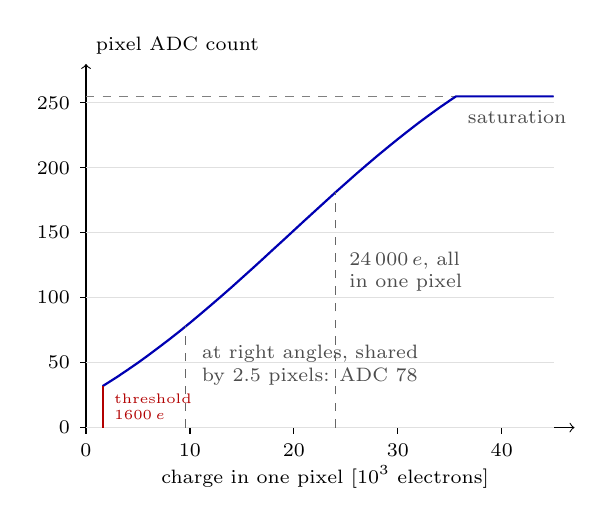
\begin{tikzpicture}[x=0.132cm, y=0.0165cm, font=\scriptsize]
\draw[->] (0,0) -- (47,0);
\node[below] at (23,-22) {charge in one pixel [$10^3$ electrons]};
\draw[->] (0,0) -- (0,280) node[above right] {pixel ADC count};
\foreach \x in {0,10,20,30,40} \draw (\x,0) -- (\x,-5) node[below] {\x};
\foreach \y in {0,50,100,150,200,250} { \draw (0,\y) -- (-0.6,\y) node[left] {\y}; \draw[black!12] (0,\y) -- (45,\y); }
\draw[black!50, dashed] (0,255) -- (45,255);
\draw[blue!70!black, thick] plot coordinates {(1.6,31.9) (2.0,33.9) (3.0,39.0) (4.0,44.4) (5.0,49.9) (6.0,55.7) (7.0,61.7) (8.0,67.8) (9.0,74.1) (10.0,80.6) (11.0,87.3) (12.0,94.1) (13.0,101.0) (14.0,108.0) (15.0,115.2) (16.0,122.4) (17.0,129.7) (18.0,137.1) (19.0,144.4) (20.0,151.8) (21.0,159.2) (22.0,166.5) (23.0,173.8) (24.0,181.1) (25.0,188.2) (26.0,195.3) (27.0,202.2) (28.0,209.0) (29.0,215.6) (30.0,222.1) (31.0,228.4) (32.0,234.6) (33.0,240.5) (34.0,246.3) (35.0,251.8) (35.6,255.0) (45.0,255.0)};
\draw[red!70!black, thick] (1.6,0) -- (1.6,31.9);
\node[red!70!black, right, align=left, font=\tiny] at (1.8,16) {threshold\\$1600\,e$};
\draw[black!60, dashed] (9.6,0) -- (9.6,78);
\node[black!70, right, align=left] at (10.2,48) {at right angles, shared\\by 2.5 pixels: ADC 78};
\draw[black!60, dashed] (24,0) -- (24,181.1);
\node[black!70, right, align=left] at (24.4,120) {$24\,000\,e$, all\\in one pixel};
\node[black!70, below right] at (35.8,252) {saturation};
\end{tikzpicture}\hfill
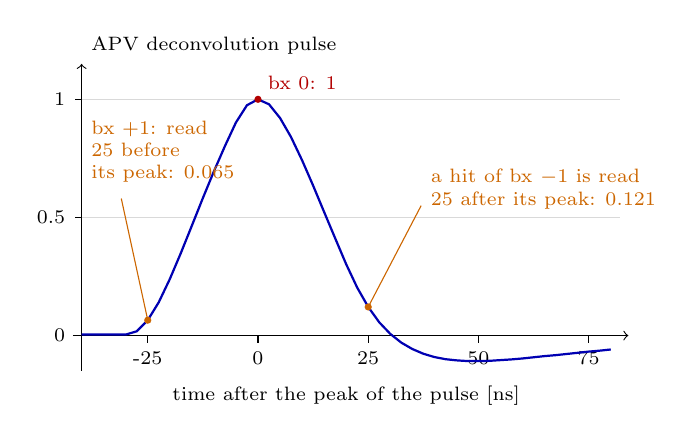
\begin{tikzpicture}[x=0.056cm, y=3.0cm, font=\scriptsize]
\draw[->] (-42,0) -- (84,0);
\node[below] at (20,-0.17) {time after the peak of the pulse [ns]};
\draw[->] (-40,-0.15) -- (-40,1.15) node[above right] {APV deconvolution pulse};
\foreach \x in {-25,0,25,50,75} \draw (\x,0) -- (\x,-0.03) node[below] {\x};
\foreach \y in {0,0.5,1} \draw (-40,\y) -- (-41.5,\y) node[left] {\y};
\draw[black!15] (-40,0.5) -- (82,0.5); \draw[black!15] (-40,1) -- (82,1);
\draw[blue!70!black, thick] plot coordinates {(-40.0,0.004) (-37.5,0.004) (-35.0,0.004) (-32.5,0.004) (-30.0,0.004) (-27.5,0.018) (-25.0,0.065) (-22.5,0.141) (-20.0,0.239) (-17.5,0.349) (-15.0,0.465) (-12.5,0.582) (-10.0,0.695) (-7.5,0.802) (-5.0,0.902) (-2.5,0.975) (0.0,1.000) (2.5,0.979) (5.0,0.921) (7.5,0.840) (10.0,0.742) (12.5,0.635) (15.0,0.523) (17.5,0.412) (20.0,0.302) (22.5,0.203) (25.0,0.121) (27.5,0.056) (30.0,0.007) (32.5,-0.030) (35.0,-0.057) (37.5,-0.077) (40.0,-0.091) (42.5,-0.100) (45.0,-0.105) (47.5,-0.108) (50.0,-0.108) (52.5,-0.107) (55.0,-0.104) (57.5,-0.101) (60.0,-0.097) (62.5,-0.092) (65.0,-0.087) (67.5,-0.083) (70.0,-0.078) (72.5,-0.073) (75.0,-0.068) (77.5,-0.064) (80.0,-0.059)};
\fill[red!70!black] (0,1) circle (1.3pt) node[above right] {bx 0: 1};
\fill[orange!80!black] (25,0.121) circle (1.3pt);
\draw[orange!80!black] (25,0.121) -- (37,0.55);
\node[orange!80!black, right, align=left] at (37,0.62) {a hit of bx $-1$ is read\\$25\ns$ after its peak: 0.121};
\fill[orange!80!black] (-25,0.065) circle (1.3pt);
\draw[orange!80!black] (-25,0.065) -- (-31,0.58);
\node[orange!80!black, right, align=left] at (-40,0.78) {bx $+1$: read\\$25\ns$ before\\its peak: 0.065};
\end{tikzpicture}
\caption{The response of the silicon readout, from the release. Left: the ADC count of a pixel as a function of its
charge, the response of \code{SiPixelDigitizerAlgorithm::missCalibrate} with the parameters of
\code{thresholds\_11\_DIGI.txt} (BPix layers 2--4 and FPix); the marks use the median charge of the signal hits,
84 electrons per $\mu$m. Right: the APV25 pulse in deconvolution mode, \code{SimTracker/SiStripDigitizer/data/APVShapeDeco\_320.txt},
by which the strip digitiser multiplies the charge of a hit according to its arrival time
(\code{SiLinearChargeDivider::TimeResponse}).}
\label{fig:11_si}
\end{figure}

\subsection{The strips}
\label{sec:11_strip}

\textbf{What it does.} The strip tracker uses the same silicon, cut into long strips some 80 to 200\,$\mu$m apart; in the
simulated geometry the sensors of the TIB and TID are 290\,$\mu$m thick, those of the TOB and of the outer TEC rings
470\,$\mu$m (the largest distance between the entry and exit points of the signal hits). Each strip is read by one
channel of an APV25 chip. The chip amplifies the charge into a pulse about $50\ns$ long and stores samples of it every
$25\ns$; in \emph{deconvolution mode}, the mode of collisions, it adds three consecutive samples with weights that undo
most of the pulse length, so that what is read for a crossing is a pulse only $25$--$30\ns$ wide on each side of its
peak (figure~\ref{fig:11_si}, right). The digitiser takes the charge of a hit, shares it among the strips it crosses,
leaks a fraction to the neighbours (cross-talk: in the inner barrel 84\,\% stays in the strip, 7\,\% goes to each
neighbour, \code{CouplingConstantRunIIDecIB1}), multiplies it by the pulse at the arrival time, and converts it at
247 electrons per ADC count. It then adds the pedestal and noise of every strip and a common-mode noise shared by the
128 strips of a chip, and applies the zero suppression of the front-end driver (FED).

\textbf{The parameters.} The FED algorithm 4 keeps a strip whose charge is above 5 times its noise, or above 2 times if
a neighbour is too (and a few rarer patterns of neighbours); the factors 5 and 2 are the payload
\code{SiStripThreshold\_Ideal\_31X\_v2}, the noise of each strip is \code{SiStripNoises}. The common-mode RMS is 5.92,
3.08, 1.08 and 2.44 ADC counts in the TIB, TID, TOB and TEC.

\begin{plainwords}[A worked example: why the strips have noise digis and the pixels none]
A particle crossing a TIB sensor at right angles frees $93.5\times290\approx27\,000$ electrons, 110 ADC counts at 247
electrons per count, shared by three strips on average: the signal digis have a median of 64 counts. The thresholds
sit at only 5 and 2 times the noise of a strip, because the strips are long and their noise large. A Gaussian
fluctuation passes 2 times the noise in 2.3\,\% of the strips; that two neighbours do so together happens about once
per thousand strips, and the strip tracker has some ten million. Hence the $12\,184$ strips without a link in the
signal sample, with a median of 18 counts and none above 85: noise that passed the zero suppression, the same in every
event whatever the collision ($12\,234$ for library event 72). The pixels, with a threshold at nine times their noise,
have none.
\end{plainwords}

\textbf{The numbers of the event.} The 8370 strip hits of the signal become $19\,418$ linked digis, 2.3 per hit, in
6473 clusters of 3.0 adjacent strips; 990 of them are at the top of the 8-bit range. In the bunch crossing the strips
make $436\,901$ digis: $19\,162$ of the signal, $279\,143$ in time, $121\,942$ early (28\,\%), 7029 late and 9625 with
no link. Why so many early ones and so few late? Figure~\ref{fig:11_si} answers half of it: a hit of bunch crossing $-1$
is read $25\ns$ after the peak of its pulse, where the pulse is still at 12\,\% of its height; one of $+1$ is read
$25\ns$ before its peak, at 6.5\,\%. The other half is the asymmetry of the pixels: a particle arrives later than light,
never earlier, so any delay moves an early hit up the falling edge (at $+20\ns$ the pulse is at 30\,\%) and a late hit
down the rising one (at $-30\ns$ it is at 0.4\,\%). Near a threshold of a few times the noise, these factors decide
whether a strip is written.

\FloatBarrier
\subsection{The ECAL and the preshower}
\label{sec:11_ecal}

\textbf{What it does.} An ECAL crystal of lead tungstate turns the energy of a shower into scintillation light, read
by avalanche photodiodes (APDs) in the barrel and vacuum phototriodes (VPTs) in the endcaps. The digitiser converts
the energy of the hits of a crystal into photoelectrons, 2250 per GeV in the barrel and 1800 in the endcaps, with
Poisson fluctuations (\code{doPhotostatistics}: $\sqrt{2250}=47$, a 2\,\% spread for a GeV), and divides them by the
\emph{laser correction} of the crystal, the fraction of light that the radiation-damaged crystal still transmits
(\code{UseLCcorrection = True}, payload \code{EcalLaserAPDPNRatios}). The light becomes a pulse of the shape stored in
the payload \code{EcalSimPulseShapePhaseI}: it rises in $50\ns$ and decays slowly, to 0.88 of its height one sample
after the peak and 0.32 four samples after it (figure~\ref{fig:11_frames}). The front-end (the MGPA amplifier and a
12-bit ADC) samples it ten times, $25\ns$ apart, with the peak of an in-time pulse in sample~6, at the highest of three
gains (12, 6, 1) that does not saturate, on a pedestal of about 200 counts with noise correlated from sample to sample.
The digitiser puts the full scale of gain 1 at $1668\GeV$ in the barrel and $2860\GeV$ in the endcaps
(\path{SimCalorimetry/EcalSimAlgos/src/EcalCoder.cc}: ``4095(MAXADC)*12(gain 2)*0.035(GeVtoADC)*0.97''), so that at
gain 12 one count is about $34\MeV$ in the barrel and $58\MeV$ in the endcaps, before the intercalibration of the
crystal, and a barrel crystal stays at gain 12 up to some $130\GeV$.

Then comes the decision that makes the ECAL different from every other subdetector: which of the $75\,848$ frames to
write. The \emph{selective readout} (\code{simEcalDigis}) reads in full the trigger towers (barrel) and supercrystals
(endcaps) that the trigger primitives flag as interesting, and applies elsewhere a zero suppression of $0.3325\GeV$ in
the barrel and $0.36\GeV$ in the endcaps to a weighted sum of the samples. Its input is the trigger primitive of every
tower, made in the same job from the unsuppressed frames; section~\ref{sec:11_tp} explains them. The preshower (ES), two
planes of silicon strips in front of the endcaps, keeps 3 samples and writes a strip whose second sample is 6 counts
above the pedestal (\code{ESThresholds\_LG\_V03\_mc}).

\begin{plainwords}[A worked example: one crystal of the $b$ jet]
The barrel crystal $(i\eta,i\phi)=(-82,239)$, at the edge of the barrel next to the $b$ jet, received $3.72\GeV$ in time.
Its frame, the largest of the signal: \code{204 201 200 200 250 265 253 241 231 219}, all at gain 12. The first three
samples are the pedestal, 201.7 on average; the pulse starts in sample 5 and peaks in sample 6, 63 counts above the
pedestal, and the samples that follow fall as the stored shape does (figure~\ref{fig:11_frames}). At $0.035\times0.97$
GeV per count a perfect crystal would give $3.72/0.034=110$ counts; this one gives 63, 17 counts per GeV. Over the 13
barrel crystals with more than $0.5\GeV$ and a frame the median is 18.4 counts per GeV instead of 29.5: the digitiser
divides the light of each crystal by its laser correction (the transparency it has lost to radiation, in the 2025
conditions) and by its intercalibration constant, and these crystals give about 0.6 of the counts of a perfect one.
The same loss weakens the trigger primitives of section~\ref{sec:11_tp}.
\end{plainwords}

\textbf{The numbers of the event.} The signal touched 5521 barrel crystals (5218 of them in time, with $67.1\GeV$),
and 156 frames are written: 100 because 4 trigger towers of 25 crystals are read in full, 56 because they passed the
zero suppression. The threshold is felt: of the crystals with more than $1\GeV$ all 6 are written, of those above
$0.3325\GeV$ 19 of 30, of those above $0.1\GeV$ 24 of 113, and 70 frames have no deposit behind them (the full-readout
towers and noise). In the endcaps, 6214 crystals with $293.7\GeV$ give 384 frames, 355 of them in the 16 supercrystals
read in full. Of the 34 endcap crystals above $1\GeV$, 19 are written, and the line between the two groups is a line in
$\eta$: the 19 are the $b$ jet, at $\abseta=1.55$--1.66; the 15 others, with up to $5.8\GeV$ each, sit at
$\abseta=2.2$--2.9, where the radiation has darkened the crystals most (the laser-monitoring ratio of the 2025
payload is 0.22 at $2<\abseta<2.5$ and 0.013 at $2.5<\abseta<3$, companion section~4.9), and a deposit of several GeV
stays under the zero suppression. Most of the $68\GeV$ the signal left in the barrel is spread over
thousands of crystals with a few MeV each, and is never read out either. In the bunch crossing the barrel writes
964 frames, the endcaps 2520 and the preshower $15\,972$ of its $137\,216$ strips (981 for the signal alone).

\begin{figure}[!htb]
\centering
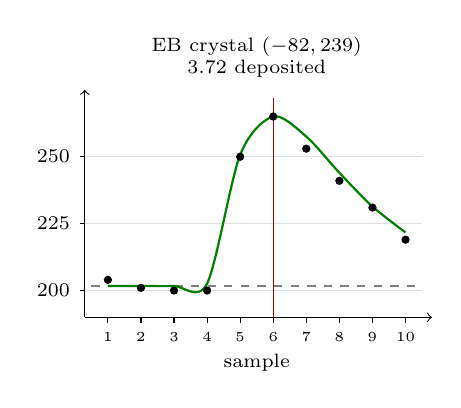
\begin{tikzpicture}[x=0.42cm, y=0.034cm, font=\scriptsize]
\node[above, align=center] at (5.5,276) {EB crystal $(-82,239)$\\$3.72\GeV$ deposited};
\draw[->] (0.3,190) -- (10.8,190);
\node[below] at (5.5,180) {sample};
\draw[->] (0.3,190) -- (0.3,275);
\foreach \x in {1,...,10} \draw (\x,190) -- (\x,188) node[below, font=\tiny] {\x};
\foreach \y in {200,225,250} { \draw (0.3,\y) -- (0.15,\y) node[left] {\y}; \draw[black!12] (0.3,\y) -- (10.5,\y); }
\draw[black!50, dashed] (0.5,201.7) -- (10.5,201.7);
\draw[red!70!black] (6,190) -- (6,272);
\draw[green!50!black, thick] plot[smooth] coordinates {(1,201.7) (2,201.7) (3,201.7) (4,202.6) (5,250.7) (6,265.0) (7,257.5) (8,244.0) (9,231.4) (10,221.7)};
\foreach \x/\y in {1/204,2/201,3/200,4/200,5/250,6/265,7/253,8/241,9/231,10/219} \fill[black] (\x,\y) circle (1.5pt);
\end{tikzpicture}\hfill
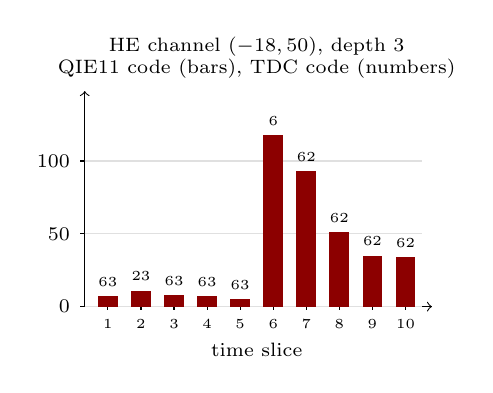
\begin{tikzpicture}[x=0.42cm, y=0.0185cm, font=\scriptsize]
\node[above, align=center] at (5.5,150) {HE channel $(-18,50)$, depth 3\\QIE11 code (bars), TDC code (numbers)};
\draw[->] (0.3,0) -- (10.8,0);
\node[below] at (5.5,-18) {time slice};
\draw[->] (0.3,0) -- (0.3,148);
\foreach \x in {1,...,10} \draw (\x,0) -- (\x,-2) node[below, font=\tiny] {\x};
\foreach \y in {0,50,100} { \draw (0.3,\y) -- (0.15,\y) node[left] {\y}; \draw[black!12] (0.3,\y) -- (10.5,\y); }
\foreach \x/\y/\t in {1/7/63,2/11/23,3/8/63,4/7/63,5/5/63,6/118/6,7/93/62,8/51/62,9/35/62,10/34/62} { \fill[red!55!black] (\x-0.3,0) rectangle (\x+0.3,\y); \node[above, font=\tiny] at (\x,\y) {\t}; }
\end{tikzpicture}\hfill
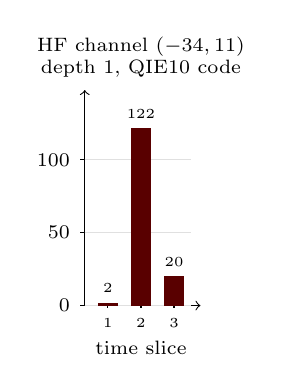
\begin{tikzpicture}[x=0.42cm, y=0.0185cm, font=\scriptsize]
\node[above, align=center] at (2,150) {HF channel $(-34,11)$\\depth 1, QIE10 code};
\draw[->] (0.3,0) -- (3.8,0);
\node[below] at (2,-18) {time slice};
\draw[->] (0.3,0) -- (0.3,148);
\foreach \x in {1,2,3} \draw (\x,0) -- (\x,-2) node[below, font=\tiny] {\x};
\foreach \y in {0,50,100} { \draw (0.3,\y) -- (0.15,\y) node[left] {\y}; \draw[black!12] (0.3,\y) -- (3.5,\y); }
\foreach \x/\y in {1/2,2/122,3/20} { \fill[red!35!black] (\x-0.3,0) rectangle (\x+0.3,\y); \node[above, font=\tiny] at (\x,\y) {\y}; }
\end{tikzpicture}
\caption{Three data frames of the signal, the largest of their kind (\code{examples\_11\_DIGI.txt}). Left: the barrel
crystal of the worked example, its ten samples (dots), the pedestal (dashed), the sample of the in-time peak (red) and
the pulse shape of the payload \code{EcalSimPulseShapePhaseI} scaled to the peak (line). Middle: the HE channel of the $b$-jet tower $(i\eta,i\phi)=
(-18,50)$, its ten QIE11 codes and, above each slice, the TDC code (63: the pulse never crossed the TDC threshold in
that slice; 62: it was already above it when the slice began; 6: it crossed $3\ns$ into the slice). Right: the HF channel of
the $\bar b$-jet tower, three slices.}
\label{fig:11_frames}
\end{figure}

\subsection{The HCAL}
\label{sec:11_hcal}

\textbf{What it does.} The barrel and endcap hadron calorimeters (HB, HE) are brass with plastic scintillator tiles;
the light of each tile is carried by fibres to a silicon photomultiplier (SiPM), and the tiles of a tower are summed
in a few \emph{depths}. The forward calorimeter (HF) is steel with quartz fibres, in which the shower makes Cherenkov
light, read by photomultipliers. The digitiser converts the visible energy of a cell into photoelectrons (for HB and HE
through the sampling factor, 125 in HB and 186 to 211 in HE, which scales the energy seen by the scintillator up to the
energy of the shower, and through the gain and the photoelectrons per femtocoulomb of the SiPM of the database; for
the HF, 6 photoelectrons per unit of the shower library of chapter~\ref{ch:10_SIM}), adds the dark current of the SiPM,
shapes the pulse and integrates it every $25\ns$ in a QIE chip (``charge integrator and encoder''). The QIE writes an
8-bit code that is not linear in the charge: two bits choose one of four ranges, six bits the step inside it, so that
the step grows with the charge. The QIE11 of HB and HE also has a TDC, which says when in the $25\ns$ the pulse crossed a
threshold, in steps of half a nanosecond (\path{SimCalorimetry/HcalSimAlgos/interface/HcalTDCParameters.h}).

\textbf{The parameters.} HB and HE write 10 time slices, with the \emph{sample of interest}, the slice of our
crossing, at 6; the HF writes 3, sample of interest 2; HO 10. The digitiser makes a frame for every channel, hit or not
(\code{doEmpty = True}), so that the noise is everywhere. The zero suppression (\code{HcalRealisticZS}) then keeps a
frame if the code of its sample of interest reaches the level of the channel in the payload
\code{HcalZSThresholds\_2025\_MOY\_mc}: 25.4 on average in HB, 9.0 in HE, 24 in HO; the HF has none.

\textbf{The numbers of the event.} The frames of figure~\ref{fig:11_frames} show what the QIE sees. The HE channel at
the heart of the $b$ jet reads codes 5 to 11 in the first five slices (pedestal and noise; the TDC answers 63, no
crossing, except for a blip at $11.5\ns$ in slice 2), jumps to 118 in slice 6 with the TDC at 6 ($3\ns$ into the slice),
and decays over the next four slices (TDC 62: still above threshold when each began). The HF channel of the
$\bar b$ jet is one slice, 122, between 2 and 20: Cherenkov light is fast. A typical kept frame is much smaller: the
median of the signal sample by its range, HE $(i\eta,i\phi)=(-16,31)$, depth 4, reads \code{4 4 5 7 6 15 12 12 15 12},
a noise fluctuation that passed the level of its channel in slice 6.

Of the $15\,840$ HB and HE frames the zero suppression keeps 4459 for the signal. The signal has hits in only 821 HB and
HE cells, so at least 3600 of the kept frames are noise; library event 72, with hits in 122 cells, keeps 4310. The
HF writes all its 3456 frames in every sample (the analyzer counts the 2270 of the signal with a positive amplitude),
and the HO none (one cell with $4\times10^{-6}\GeV$). In the bunch crossing the zero suppression keeps 6545 HB/HE frames,
2 HO frames, and the summed amplitudes grow from the signal alone by a factor 1.7 in the HB, 7.0 in the HE and 3.7 in
the HF.

\FloatBarrier
\subsection{The muon chambers}
\label{sec:11_muon}

\textbf{What it does.} Four technologies, four digitisers, each a module of its own after the mixing
(\path{SimMuon/Configuration/python/SimMuon_cff.py}). The \emph{drift tubes} (DT) of the barrel record, for each wire,
the time at which the electrons of the track arrived after drifting across the cell; the drift velocity is about
$55\,\mu$m/ns (the constant of the ideal model of the digitiser), so the time is a distance, and it runs to hundreds of
nanoseconds. The digitiser adds a fixed offset of $500\ns$ (\code{pset.offset}), a smearing of $2.4\ns$ and a dead
time of $150\ns$ per wire, and counts in TDC units of $25/32\ns$. The \emph{cathode strip chambers} (CSC) of the
endcaps have six layers of wires and strips: a strip records 8 samples of its pulse, $50\ns$ apart, with the peak in
sample 5, and is read with the whole front-end board of 16 strips it belongs to, plus the neighbouring board if the hit
is within 3 strips of its edge (\code{CSCStripElectronicsSim::channelsToRead}); a wire group records the time bin of its
pulse. The \emph{resistive plate chambers} (RPC) and the \emph{GEM} chambers in front of the first endcap station are
fast: a strip and a bunch crossing.

\textbf{The parameters.} The pedestals, gains and noise of the CSC strips are read from the database
(\code{stripConditions} is \code{Database}; the \code{pedestal = 600} of the python is used only with the configurable conditions). The RPC have an
efficiency of 0.95 and a noise and background model (\code{doBkgNoise = True}), the GEM an efficiency of 0.98 and no
noise.

\textbf{The numbers of the event.} The signal reaches no chamber: its only muon digis are 8 RPC strips of the noise
model. Library event 72 has 11 CSC hits (a forward particle reaching ME1), and they give 176 strip digis of which 18
are linked: the other 158 are the rest of the boards read with them. In the bunch crossing the chambers have 2016 digis
(figure~\ref{fig:11_rz}). The 12 DT digis have times between 564 and $922\ns$, 64 to $422\ns$ once the offset is
taken away; 9 of
them come from bunch crossing $-1$: a wire still collects the electrons of a track $25\ns$ older, and more. The 1888
CSC strip digis sit in 13 chambers, 96 to 256 each, always whole boards of 16 strips (6 to 16 boards): 305 are
linked to an in-time particle, 62 to an early one and 36 to a late one, and the 1485 others are their board neighbours,
flat at the pedestal (the median strip moves by 5 counts over its 8 samples; the largest pulse, in ME1/1, goes from 1016
to 2232). Four of the 13 chambers, ME1/1 chamber 20, ME2/1 chamber 10, ME3/1 and ME4/1 chamber 11 of the negative
endcap, are crossed by the one pileup muon that the Level-1 trigger of chapter~\ref{ch:12_L1T} will find. The 91 wire
digis have time bins 6 to 12, most of them 8; the 10 RPC digis bunch crossings $-3$ to $+4$ (7 without a link); the 15
GEM digis bunch crossings $-1$ to $+1$.

\begin{figure}[!htb]
\centering
\includegraphics[width=0.86\textwidth]{11_DIGI/out/digiAnalyzer_mixed_11_DIGI_rz_run1_event1.png}
\caption{The bunch crossing digitised, in $r$--$z$. The tracker
($r<1.2$\,m) is solid with in-time (blue) and early (orange) pileup digis; the green bars are the ECAL frames, the red
triangles the HCAL frames (dark red at $|z|\approx11$\,m: the HF), most of them noise that passed the zero suppression.
Outside, the muon digis: the CSC chambers of the endcaps (left and right, $|z|=5.8$ to $10.1$\,m), the DT wires of the
barrel ($r=4$ to 7\,m), grey where no particle is linked to them. The right panel has the exact counts
(\code{digiAnalyzer\_mixed\_11\_DIGI\_rz\_run1\_event1.png}).}
\label{fig:11_rz}
\end{figure}

\subsection{The three samples side by side}
\label{sec:11_samples}

\textbf{(11a) The signal alone.} $44\,172$ digis. In the tracker $36\,402$, of which $24\,218$ linked to a signal
particle and $12\,184$ strip noise; the pixels have no noise digi. In the calorimeters 156 EB, 384 EE and 981 ES frames
and 4459 HB/HE frames, most of them noise. In the muon chambers 8 RPC noise strips. In figure~\ref{fig:11_alone} (left)
the $b$ jet at $(\eta,\phi)=(-1.6,-2.1)$ is a dense patch of black tracker digis under large green EB frames and the
$\bar b$ jet at $\eta=-3.75$ sits in the HF ring beyond the tracker.

\textbf{(11b) One collision alone.} Library event 72 is an ordinary inelastic collision: 2097 tracker hits, 5270
linked digis, and $12\,234$ noise strips, as many as the signal sample, so that its $17\,504$ tracker digis are
70\,\% noise. The ECAL keeps 43 EB and 105 EE frames (three supercrystals read in full), the ES 360; the HCAL zero
suppression keeps 4310 HB/HE frames. The right panel of figure~\ref{fig:11_alone} is what a bunch crossing's worth of
pileup looks like one collision at a time.

\textbf{(11a+11b) The signal with its bunch crossing.} $544\,407$ digis. The \code{DigiSimLink}s sort the $514\,881$ tracker
digis: $23\,765$ signal (4.6\,\%), $350\,718$ in-time pileup (68\,\%), $123\,744$ early (24\,\%), 7029 late (1.4\,\%),
9625 without a link. A channel that two particles share is attributed to the one with the larger charge fraction, and
the signal lost 453 of its $24\,218$ digis this way. The 68 in-time collisions give 5158 digis each, so that the signal
weighs as much as 4.6 of them. In the calorimeters there is no sorting: one frame per channel, and the summed
amplitudes grow from the signal alone to the bunch crossing by a factor 7.1 in the EB (1260 to 8899 counts), 6.5 in the
EE (1876 to $12\,194$), 12.9 in the ES, 1.7 in the HB, 7.0 in the HE ($20\,375$ to $141\,702$) and 3.7 in the HF. The
selective readout now reads 23 barrel towers and 100 of the 624 endcap supercrystals in full, and the EE frames go
from 384 to 2520.

\begin{figure}[htb]
\centering
\begin{subfigure}[t]{0.49\textwidth}
\includegraphics[width=\textwidth]{11_DIGI/out/digiAnalyzer_signal_11_DIGI_etaphi_run1_event1.png}
\caption{(11a) the signal alone: $44\,172$ digis, $24\,218$ tracker digis linked to the signal, $12\,184$ tracker noise.}
\end{subfigure}\hfill
\begin{subfigure}[t]{0.49\textwidth}
\includegraphics[width=\textwidth]{11_DIGI/out/digiAnalyzer_pileup_11_DIGI_etaphi_run1_event72.png}
\caption{(11b) library event 72 alone: $24\,104$ digis, 5288 linked to the collision, $12\,403$ noise.}
\end{subfigure}
\caption{The digis of the signal alone and of one pileup collision alone, $\eta$--$\phi$ from the signal vertex.
Black: tracker and muon digis linked to the sample's own particles, grey: no link (noise); green squares: ECAL frames
sized by their amplitude above pedestal (light green: ES); red triangles: HCAL (dark red: HF); magenta circles: the
signal \code{ak4GenJets} above $30\GeV$ (\code{digiAnalyzer\_signal\_11\_DIGI\_etaphi\_run1\_event1.png},
\code{digiAnalyzer\_pileup\_11\_DIGI\_etaphi\_run1\_event72.png}).}
\label{fig:11_alone}
\end{figure}

\subsection{What the year changed}
\label{sec:11_year}

The same job on the 2024 global tag (companion, section~4.9) had the same hits and collisions, and other digis. The
python of the digitisers is identical with both eras; what changed are payloads of the global tag. The signal made 4982
linked pixel digis there and 4800 here: the Lorentz angle of the 2025 simulation is smaller (0.036 instead of 0.071 per
tesla in the first barrel layer), the charge spreads over fewer pixels. The barrel ECAL wrote 399 frames for the signal
and 2050 for the bunch crossing, now 156 and 964: the zero suppression of a low-interest barrel tower went from
$0.2275$ to $0.3325\GeV$ (6.5 to 9.5 counts of the $35\MeV$ unit of the selective readout,
\code{EcalSRSettings\_2024\_EBZS9.5\_EEZS6.0\_DCC2\_mc}), the crystals give less light (the laser correction of the
worked example) and their noise is larger (a pedestal width of 3.31 instead of 2.85 counts). The HCAL keeps 4459 HB/HE
frames for the signal instead of 3285: the SiPMs of 2025 have twice the dark current (HB: 14.9 instead of
$7.7\,\mu$A), and noise is what most kept frames are. The rest differs little, and by chance (the digitisers share one
random engine); the trigger primitives changed most.

\section{Made here for the next stage: the trigger primitives}
\label{sec:11_tp}

\textbf{What they are.} Two of the products listed above are not digis in the sense of this chapter:
\code{simEcalTriggerPrimitiveDigis} and \code{simHcalTriggerPrimitiveDigis}. Nobody will reconstruct the event
from them. A \emph{trigger primitive} is the message that a calorimeter sends, every 25\,ns, to the Level-1 trigger
of chapter~\ref{ch:12_L1T}: one transverse energy for a whole \emph{trigger tower}, on 8 bits, with a few flag bits.
The data frames of this chapter cannot play that role. They are read out only \emph{after} the trigger has said
yes, there are $75\,848$ ECAL crystals with ten samples each, and the trigger has about four microseconds. So each
calorimeter has a second output in parallel with its data frames: coarse (one number for 25 crystals, or for all the
depths of an HCAL tower), fast (computed for every bunch crossing, whether anything happened or not) and lossy.
It is all the Level-1 trigger will ever know of the calorimeters.

\begin{plainwords}[The grid of the calorimeter trigger]
The trigger sees the calorimeters as towers numbered by two integers, $i\eta=\pm1\ldots\pm41$ (no 0) and
$i\phi=1\ldots72$. In the barrel a tower is $5\times5$ ECAL crystals and the HCAL tower behind them,
$0.087\times0.087$ in $\eta\times\phi$ ($5^\circ$ in $\phi$). The barrel ECAL ends at $|i\eta|=17$, the barrel HCAL
at 16, the endcaps at 28; towards the endcap edge the towers grow in $\eta$ (tower 28 covers
$2.65<\abseta<3.0$, four times the area of a barrel tower); $|i\eta|=29$ is not used; 30 to 41 are the HF,
$3.0<\abseta<5.2$, where a primitive is $10^\circ$ wide in $\phi$ ($20^\circ$ for $|i\eta|\geq40$). In all
$2\times28\times72=4032$ ECAL primitives, 4032 for HB and HE, and 792 for the HF: 8856 numbers per bunch crossing,
each an integer count of $0.5\GeV$ of transverse energy, at most 255 counts ($127.5\GeV$).
\end{plainwords}

\textbf{How they are made.} In the ECAL (\code{EcalTrigPrimProducer}; the classes of
\path{SimCalorimetry/EcalTrigPrimAlgos} are named after the FENIX chips of the front-end they emulate) the samples
of each crystal are linearised and the five crystals of a strip are summed; an amplitude filter with fixed weights
turns the samples into a pulse height and a peak finder keeps it only in the crossing where it is maximal
(\code{binOfMaximum = 6}, where the digitiser puts the maximum of an in-time pulse, figure~\ref{fig:11_frames}); the
five strips of a tower are added, and a lookup table converts the sum to the 8-bit $E_{\mathrm T}$ and to a
\emph{trigger-tower flag}: low, mid or high interest. A fine-grain bit says whether the energy sits in two adjacent
strips, as for an electron or a photon. The weights, pedestals, linearisation constants and thresholds are nineteen
payloads of the global tag (\code{EcalTPG*Rcd}). In the HCAL (\code{HcalTrigPrimDigiProducer}) the charge of every
depth of a tower is linearised with a per-channel lookup table (with $1/16\GeV$ per count), the depths are summed, the
time samples are combined with database weights that can subtract the tail of the previous crossing, a peak finder
picks the crossing (\code{PeakFinderAlgorithm = 2}) and the result is compressed to 8 bits, since 2018 linearly,
$0.5\GeV$ per count; six feature bits (depth profile and timing) go with it. In the HF the long and the short fibres
of a tower are summed over two samples. The parameters of the two producers are in \path{thresholds_11_DIGI.txt}.

\textbf{Why they are made in the DIGI job, when the Level-1 trigger is the next chapter.} For three reasons, the
first of which leaves no choice.
\emph{(1) Their input does not survive this job.} The primitives are computed from the \emph{unsuppressed} frames:
every crystal, every sample, noise included (\code{Label = simEcalUnsuppressedDigis}). Those frames exist only
between the digitiser and the selective readout; the event content keeps the HCAL ones but not the ECAL barrel and
endcap ones (\path{SimCalorimetry/Configuration/python/SimCalorimetry_EventContent_cff.py}), and the 964 barrel
frames that this chapter wrote out of $61\,200$ are not enough to recompute a tower sum. After the DIGI job the
ECAL primitive cannot be made any more.
\emph{(2) The DIGI job itself needs them.} The selective readout of the ECAL, which decides what
this chapter wrote, is driven by the trigger-tower flags: \code{simEcalDigis} has
\code{trigPrimProducer = simEcalTriggerPrimitiveDigis}, and the task is written in that order with the comment
``ECAL Trigger Primitives (needed by SRP)'' (\path{SimCalorimetry/Configuration/python/ecalDigiSequence_cff.py}). The
trigger primitive is an \emph{input} of the ECAL digis, not a by-product.
\emph{(3) It is where they are made in the detector.} The primitive is computed by the electronics of each
calorimeter, the electronics this chapter simulates, not by the trigger, and it is part of the data: the
\code{DIGI2RAW} step packs it with the frames (\path{EventFilter/EcalDigiToRaw/python/ecalDigiToRaw_cfi.py},
\code{labelTT}). In the production DIGI, L1 and DIGI2RAW are one job and the seam does not show; this book cuts
the journey into stages, and the cut between this chapter and the next passes \emph{behind} the trigger primitives. The muon chambers are the opposite case:
their trigger primitives are made from the stored muon digis by the L1 step itself, and belong to
chapter~\ref{ch:12_L1T}.

\textbf{The numbers of the event.} The three samples of this chapter exist for the last time: from
chapter~\ref{ch:12_L1T} on, only the signal with its pileup is followed. Table~\ref{tab:11_tp} counts their
primitives (the analyzer \code{TrigPrimAnalyzer}, \path{test/11_DIGI/out/trigprim_11_DIGI.txt}).

\begin{table}[!htb]
\centering\small\setlength{\tabcolsep}{4pt}
\caption{The trigger primitives with $E_{\mathrm T}>0$, their summed $E_{\mathrm T}$ and the largest one
(\code{trigprim\_11\_DIGI.txt}, section 1), out of 2448 (EB), 1584 (EE), 2304 (HB), 1728 (HE) and 792 (HF).}
\label{tab:11_tp}
\begin{tabular}{l rrr c rrr c rrr}
\toprule
 & \multicolumn{3}{c}{(11a) signal alone} & & \multicolumn{3}{c}{(11b) event 72 alone} & & \multicolumn{3}{c}{(11a+11b) signal + pileup} \\
\cmidrule(lr){2-4}\cmidrule(lr){6-8}\cmidrule(lr){10-12}
 & $>0$ & $\sum E_{\mathrm T}$ & max & & $>0$ & $\sum E_{\mathrm T}$ & max & & $>0$ & $\sum E_{\mathrm T}$ & max \\
 & & [GeV] & [GeV] & & & [GeV] & [GeV] & & & [GeV] & [GeV] \\
\midrule
ECAL barrel (EB) & 368 & 215.0 & 3.0 & & 340 & 185.0 & 1.5 & & 683 & 468.0 & 5.5 \\
ECAL endcap (EE) & 131 & 113.5 & 6.0 & & 105 & 69.0 & 3.0 & & 494 & 579.5 & 7.0 \\
HCAL barrel (HB) & 69 & 35.5 & 1.5 & & 51 & 26.0 & 1.0 & & 233 & 183.0 & 7.5 \\
HCAL endcap (HE) & 12 & 24.0 & 10.0 & & 0 & 0.0 & -- & & 328 & 241.5 & 10.0 \\
HF & 40 & 148.5 & 89.0 & & 4 & 2.0 & 0.5 & & 741 & 1321.0 & 90.5 \\
\midrule
all & 620 & 536.5 & 89.0 & & 500 & 282.0 & 3.0 & & 2479 & 2793.0 & 90.5 \\
\bottomrule
\end{tabular}
\end{table}

\emph{What a primitive measures.} For the ECAL the file still holds the energy that the particles left in the
crystals (the \code{PCaloHit}s of chapter~\ref{ch:10_SIM}), and the analyzer sums it per trigger tower as transverse
energy. The signal alone left $120.7\GeV$ of $E_{\mathrm T}$ in 2799 of the 4032 ECAL towers. In the 32 towers where
it left at least a quarter of a GeV and a primitive was sent, the deposits add up to $49.8\GeV$ and the primitives
to $48.0\GeV$: the primitive is the transverse energy of the tower, to a few per cent. But $52.6\GeV$ are spread over
some 2700 towers with less than $0.25\GeV$ each, and 41 towers with $18.3\GeV$ fall just short of one count: for
these the primitive is zero. More than half of what the signal deposited in the ECAL is invisible to the trigger.

\emph{Most ECAL primitives are noise.} The signal alone sends 499 ECAL primitives; 467 of them, $280.5\GeV$, come
from towers where it deposited less than $0.25\GeV$. Library event 72 deposited $14.6\GeV$ of $E_{\mathrm T}$ in
the whole ECAL, in only four towers as much as a quarter of a GeV, and still sends 445 primitives, $254.0\GeV$, the
largest $3\GeV$: the sum of 25 noisy crystals fluctuates up to a count in one tower in nine. No particle is behind
these numbers, and every step of the Level-1 trigger will need a threshold because of them. (In 2024 it was one
tower in seventeen; the barrel crystals of 2025 are noisier, a pedestal width of 3.31 instead of 2.85 ADC counts.)

\emph{One primitive per bunch crossing.} A primitive digi stores a few consecutive crossings, and their sums show
that the calorimeters talk to the trigger continuously (\code{trigprim\_11\_DIGI.txt}, section 2). For the signal
alone the ECAL sends 426.5, 268.5, [328.5], 274.0 and $280.0\GeV$ in crossings $-2$ to $+2$: some $270\GeV$ of
noise in every crossing, and $60\GeV$ more in ours. With the pileup it sends 517.5, 826.0, [1047.5], 575.5 and
$190.5\GeV$, and the HB and HE 34.0, 255.5, [424.5] and $350.0\GeV$: the crossings $-1$ and $+1$, with their 71 and
54 collisions, are events of their own for the trigger, which will judge each of them separately.

\emph{The primitives decide what the ECAL reads out.} A tower with a primitive of at least $2\GeV$ is flagged mid
interest, of at least $4\GeV$ high interest (the payload is
\path{EcalTPGPhysicsConst_2025_mc_EB_4.0_2.0_EE_4.0_2.0}). The signal alone has four barrel towers flagged mid
($2$ to $3\GeV$) and none high: these are exactly the four barrel towers that the selective readout read in
full (section~\ref{sec:11_ecal}), and only one of them, $(-17,46)$, is on the $b$ jet; the other three are noise. With
the pileup there are 14 mid towers and one high ($5.5\GeV$ at $(i\eta,i\phi)=(-4,4)$): a mid tower is read in full
alone, a high one with its eight neighbours, $14+9=23$ towers, the number found above. In the endcap 76 mid and 13 high
towers give the 100 supercrystals (2024: 175): the endcap crystals of 2025 have lost more transparency (at
$2.5<\abseta<3$ the digitiser scales their light by 0.013 instead of 0.041), and the primitives do not make up for
it. Every full-readout decision of this chapter was taken by a trigger primitive.

\emph{The two jets.} Figures~\ref{fig:11_tp} and~\ref{fig:11_tphf} show the primitives of the signal alone and of the
signal with its pileup, and the two jets tower by tower. The $\bar b$ jet, in the HF, is narrow: one primitive
of $89.0\GeV$ at $i\eta=-34$, and $123.75\GeV$ in the $9\times9$ towers around the jet axis. The $b$ jet, on the
barrel--endcap boundary, is spread out: a column of ECAL towers at $i\eta=-19$ with $6.0$ and $5.5\GeV$
and three HCAL towers with $10.0$, $4.0$ and $3.5\GeV$; around its axis the ECAL
primitives hold $29.0\GeV$ of the $41.6\GeV$ deposited there and the HCAL ones $22.5\GeV$. With the pileup the
same windows hold $78.5\GeV$ for the $b$ jet and $199.75\GeV$ for the $\bar b$ jet: the pileup adds $27\GeV$ to
one and $76\GeV$ to the other, and it lights up the HF and the endcap ECAL. In the HF (figure~\ref{fig:11_tphf}) the
largest primitive barely moves, 89.0 to $90.5\GeV$, but the towers around it, empty or nearly so for the signal alone,
now hold half a GeV to a few GeV each. This is the event chapter~\ref{ch:12_L1T} receives: 2479 primitives, $2793.0\GeV$. The
signal alone sent $536.5\GeV$, a fifth of it, but more than half of that was its own noise.

\begin{figure}[!htb]
\centering
\includegraphics[width=0.325\textwidth,trim=0 0 475 0,clip]{11_DIGI/out/trigPrim_signal_11_DIGI_ecaltp_run1_event1.png}\hfill
\includegraphics[width=0.325\textwidth,trim=0 0 475 0,clip]{11_DIGI/out/trigPrim_signal_11_DIGI_hcaltp_run1_event1.png}\hfill
\includegraphics[width=0.325\textwidth,trim=0 0 475 0,clip]{11_DIGI/out/trigPrim_signal_11_DIGI_jet1_ecaltp_run1_event1.png}\\[2pt]
\includegraphics[width=0.325\textwidth,trim=0 0 475 0,clip]{11_DIGI/out/trigPrim_mixed_11_DIGI_ecaltp_run1_event1.png}\hfill
\includegraphics[width=0.325\textwidth,trim=0 0 475 0,clip]{11_DIGI/out/trigPrim_mixed_11_DIGI_hcaltp_run1_event1.png}\hfill
\includegraphics[width=0.325\textwidth,trim=0 0 475 0,clip]{11_DIGI/out/trigPrim_signal_11_DIGI_jet1_hcaltp_run1_event1.png}
\caption{The trigger primitives (\code{trigPrim\_<case>\_11\_DIGI\_*.png}). Left and middle columns: the ECAL and
the HCAL primitives (with the HF beyond $\abseta=3$) on the trigger-tower grid, one coloured cell per tower, colour
= $E_{\mathrm T}$ on a logarithmic scale from $0.25$ to $256\GeV$; top (11a) the signal alone, bottom (11a+11b) the
signal with its pileup; magenta circles: the two \code{ak4GenJets}. Right column: the $b$ jet of the signal alone
tower by tower, ECAL (top) and HCAL (bottom) primitives of the $17\times17$ towers around the jet axis with their
$E_{\mathrm T}$ in GeV; black: the tower of the axis, $(i\eta,i\phi)=(-19,49)$; red: the $9\times9$ towers around
it, the size of a Level-1 jet.}
\label{fig:11_tp}
\end{figure}

\begin{figure}[!htb]
\centering
\includegraphics[width=0.47\textwidth,trim=0 0 475 0,clip]{11_DIGI/out/trigPrim_signal_11_DIGI_jet2_hcaltp_run1_event1.png}\hfill
\includegraphics[width=0.47\textwidth,trim=0 0 475 0,clip]{11_DIGI/out/trigPrim_mixed_11_DIGI_jet2_hcaltp_run1_event1.png}
\caption{The $\bar b$ jet in the HF, the HCAL primitives of the $17\times17$ towers around its axis $(i\eta,i\phi)=(-34,12)$
(\code{trigPrim\_signal/mixed\_11\_DIGI\_jet2\_hcaltp\_run1\_event1.png}). Left: the signal alone, $123.75\GeV$ in the
$9\times9$ window (red); right: with its pileup, $199.75\GeV$. An HF primitive is two towers wide in $\phi$ (grey
frames); the column at $i\eta=-28$ is the last ring of the endcap.}
\label{fig:11_tphf}
\end{figure}

\FloatBarrier
\section{Ledger and display}

Table~\ref{tab:11_ledger} is the ledger of the stage: what went into each digitiser and what came out, for the three
samples. The stage does not add or remove energy in the sense of the generator chapters; it changes the currency. The
tracker hits come out as pixels and strips, 3.5 per hit for the signal, 1.1 per hit for the bunch crossing (most of
the out-of-time hits fall outside the windows); the calorimeter cells go in with an energy in GeV (or shower-library
units in the HF) and come out as data frames with an amplitude in ADC counts, and only a fraction of the cells with a
hit becomes a digi (EB: 5521 cells, 156 digis for the signal). The noise is the one entry the stage adds: $12\,184$
tracker strips and at least 3600 HB/HE frames appear where nothing crossed the channel.

\begin{table}[tb]
\centering\scriptsize\setlength{\tabcolsep}{2.5pt}
\caption{The ledger of the digitisation (\code{ledger\_11\_DIGI.txt}; the SimHits of the signal from
\code{test/10\_SIM/out/simHits\_signal\_10\_SIM.log}, of the bunch crossing from \code{step3\_MIX\_10\_SIM.log}, of library
event 72 and the HCAL cells from the FWLite extras of the companion). Top: tracker and muon chambers, hits in and digis
out, the digis split by their \code{DigiSimLink}; for the bunch crossing the hits per subdetector are the sum of the
\code{CrossingFrame} (signal and all pileup). Bottom: calorimeters, cells with a hit and their energy in, data frames
and their summed amplitude above pedestal (ADC counts) out.}
\label{tab:11_ledger}
\begin{tabular}{lrrrrcrrrrcrrrrrrr}
\toprule
 & \multicolumn{4}{c}{(11a) signal alone} & & \multicolumn{4}{c}{(11b) library event 72 alone} & & \multicolumn{7}{c}{(11a+11b) signal + 71 / 68 / 54 collisions} \\
\cmidrule(lr){2-5}\cmidrule(lr){7-10}\cmidrule(lr){12-18}
 & hits & digis & linked & noise & & hits & digis & linked & noise & & hits & digis & signal & in-time & early & late & noise \\
\midrule
PXB & 929 & 3011 & 3011 & 0 & & 277 & 819 & 819 & 0 & & 50\,953 & 52\,101 & 2824 & 47\,941 & 1336 & 0 & 0 \\
PXF & 973 & 1789 & 1789 & 0 & & 176 & 318 & 318 & 0 & & 36\,700 & 25\,879 & 1779 & 23\,634 & 466 & 0 & 0 \\
TIB & 1182 & 5360 & 3120 & 2240 & & 187 & 2841 & 555 & 2286 & & 71\,941 & 91\,364 & 3077 & 60\,025 & 25\,030 & 1530 & 1702 \\
TID & 975 & 2558 & 1774 & 784 & & 172 & 1141 & 339 & 802 & & 37\,897 & 34\,922 & 1730 & 24\,228 & 7759 & 692 & 513 \\
TOB & 1022 & 6778 & 2798 & 3980 & & 209 & 4448 & 541 & 3907 & & 69\,140 & 106\,837 & 2761 & 62\,356 & 37\,048 & 1220 & 3452 \\
TEC & 5191 & 16\,906 & 11\,726 & 5180 & & 1076 & 7937 & 2698 & 5239 & & 181\,684 & 203\,778 & 11\,594 & 132\,534 & 52\,105 & 3587 & 3958 \\
\midrule
tracker & 10\,272 & 36\,402 & 24\,218 & 12\,184 & & 2097 & 17\,504 & 5270 & 12\,234 & & 448\,315 & 514\,881 & 23\,765 & 350\,718 & 123\,744 & 7029 & 9625 \\
\midrule
DT & 0 & 0 & 0 & 0 & & 0 & 0 & 0 & 0 & & -- & 12 & 0 & 1 & 9 & 2 & 0 \\
CSC strip & 0 & 0 & 0 & 0 & & 11 & 176 & 18 & 158 & & -- & 1888 & 0 & 305 & 62 & 36 & 1485 \\
CSC wire & 0 & 0 & 0 & 0 & & 11 & 3 & 0 & 3 & & -- & 91 & 0 & 0 & 0 & 0 & 91 \\
RPC & 0 & 8 & 0 & 8 & & 0 & 8 & 0 & 8 & & -- & 10 & 0 & 3 & 0 & 0 & 7 \\
GEM & 0 & 0 & 0 & 0 & & 0 & 0 & 0 & 0 & & -- & 15 & 0 & 14 & 1 & 0 & 0 \\
\bottomrule
\end{tabular}

\medskip
\begin{tabular}{lrrrrcrrrrcrrr}
\toprule
 & \multicolumn{4}{c}{(11a) signal alone} & & \multicolumn{4}{c}{(11b) library event 72 alone} & & \multicolumn{3}{c}{(11a+11b)} \\
\cmidrule(lr){2-5}\cmidrule(lr){7-10}\cmidrule(lr){12-14}
 & cells & $E$ in & digis & ADC out & & cells & $E$ in & digis & ADC out & & digis & ADC out & ratio to (11a) \\
\midrule
EB & 5521 & 68.0\,GeV & 156 & 1260 & & 1217 & 9.4\,GeV & 43 & 502 & & 964 & 8899 & 7.1 \\
EE & 6214 & 293.7\,GeV & 384 & 1876 & & 1948 & 43.5\,GeV & 105 & 384 & & 2520 & 12\,194 & 6.5 \\
ES & 1069 & 0.25\,GeV & 981 & 17\,885 & & 223 & 0.05\,GeV & 360 & 5053 & & 15\,972 & 230\,844 & 12.9 \\
HB & 173 & 0.22\,GeV & 1722 & 16\,684 & & 21 & 0.02\,GeV & 1700 & 15\,856 & & 2197 & 29\,111 & 1.7 \\
HE & 648 & 1.66\,GeV & 2249 & 20\,375 & & 101 & 0.22\,GeV & 2036 & 12\,739 & & 3966 & 141\,702 & 7.0 \\
HO & 1 & $4\times10^{-6}$\,GeV & 0 & 0 & & 0 & 0 & 0 & 0 & & 2 & 63 & -- \\
HF & 531 & 1849 units & 2270 & 8234 & & 119 & 173 units & 2169 & 4167 & & 1889 & 30\,729 & 3.7 \\
\midrule
all digis & & & 44\,172 & & & & & 24\,104 & & & 544\,407 & & \\
\bottomrule
\end{tabular}
\end{table}

Figure~\ref{fig:11_mixed} is the $\eta$--$\phi$ display of the event at the end of the journey. The tracker region,
$\abseta<2.5$, is solid with the $350\,718$ blue in-time and $123\,744$ orange early pileup digis; the $23\,765$ black
signal digis are drawn on top and are visible as a darker patch only inside the $b$-jet circle at $(-1.6,-2.1)$. The
green ECAL frames show the same thing in energy: the $b$ jet is still the largest cluster of the barrel, but the
endcaps, $1.5<\abseta<3$, are now a wall of green, 2520 EE frames against 384 for the signal, and the ES ($15\,972$
strips) fills the same band. The HF ring, where the $\bar b$ jet of $114\GeV$ fell in chapter~\ref{ch:10_SIM}, has
the same number of frames as before (every channel is read) with nearly four times the amplitude. Compared with page 6 of
chapter~\ref{ch:09_G4}, where the event was 571 coloured dots and two circles, the two circles are the only thing
that is still recognisable.

\begin{figure}[tb]
\centering
\includegraphics[width=0.8\textwidth]{11_DIGI/out/digiAnalyzer_mixed_11_DIGI_etaphi_run1_event1.png}
\caption{The signal with its bunch crossing digitised:
$544\,407$ digis, the tracker and muon digis coloured by their link (black: signal, blue: in-time pileup, orange:
bunch crossing $-1$, red: $+1$, grey: no link), the ECAL (green) and HCAL (red) frames sized by amplitude, the two
signal jets as magenta circles. The tracker and muon digis are thinned for the drawing (at most 8000 per
subdetector); the counts in the right panel are exact (\code{digiAnalyzer\_mixed\_11\_DIGI\_etaphi\_run1\_event1.png}). The
$r$--$z$ page of the same PDF is figure~\ref{fig:11_rz}.}
\label{fig:11_mixed}
\end{figure}

What is left of the signal: in the tracker 4.6\,\% of the digis, and the \code{DigiSimLink}s know which; in the
calorimeters nothing is labelled, the EE frame of a crystal in the $\bar b$ direction holds the sum of the signal
pulse and of the pulses of 193 collisions, sampled ten times. From here on the separation is the job of the
reconstruction, with three handles: the position (a jet is narrow, the pileup is flat in $\eta$--$\phi$), the
vertex (the tracker links the charged part of a jet to one $z$) and the time (the out-of-time pileup peaks in a
different sample). The $\bar b$ jet, at $\eta=-3.75$, beyond the tracker, has only the first of the three.

\section{Open problems for Phase-2}

The Phase-2 era of this release is \code{Phase2C17I13M9}, defined in
\path{Configuration/Eras/python/Era_Phase2C17I13M9_cff.py} as the \code{Phase2} chain (\code{phase2\_common},
\code{phase2\_tracker}, \code{phase2\_hgcal}, \code{phase2\_timing\_layer}, \code{phase2\_muon}) plus \code{phase2\_GE0}
and the HGCal V10--V16 modifiers. It rebuilds \code{process.mix.digitizers} in
\path{SimGeneral/MixingModule/python/digitizers_cfi.py}: the strip digitiser is removed, the pixel one replaced by
the \code{Phase2TrackerDigitizer}, the HGCal and MTD digitisers added, the ECAL endcap and preshower switched off.

\textbf{The Phase-2 tracker digitiser carries 2012 numbers.} In \path{SimTracker/SiPhase2Digitizer/python/phase2TrackerDigitizer_cfi.py}
the inner pixels have a threshold of 1000\,e without smearing (\code{AddThresholdSmearing = False}), no noise
(\code{NoiseInElectrons = 0}, \code{AddNoise = False}, \code{AddNoisyPixels = False}), no inefficiency, 1500\,e per
ADC count on 4 bits (\code{AdcFullScale = 15}, dual-slope readout mode 3) and a time window of $-5$ to $+20\ns$;
against the 1600\,e, 245\,e smearing, 175\,e noise, 8 bits and $\pm12.5\ns$ of table~\ref{tab:11_cuts}, the HL-LHC
pixel is simulated without noise, noisy pixels or inefficiency, and \code{UseReweighting = False} carries the comment
``will be True for realistic simulations''. The outer-tracker modules have thresholds of 6300\,e (PS pixels, ``0.4
MIP''), 4800\,e (PS strips) and 6000\,e (2S) with noise 1010 and 1263\,e set so that ``4.75 sigma $\Rightarrow$
occupancy = 1e-6'', a square-window hit detection (\code{HitDetectionMode = 0}), \code{CBCDeadTime = 0},
\code{KillModules = False} and a charge-sharing parameter \code{SigmaCoeff} ``to be confirmed with simulations in
CMSSW\_6.X''. The bias-rail inefficiency, the dead strips and the pixel time-walk exist only as customisations
(\path{customizeForOTInefficiency.py}, \path{customizeForPhase2TrackerSignalShape.py}). In the Run-3
digitiser the radiation damage of the pixels enters through the DB templates (\code{UseReweighting = True} under
\code{phase1Pixel} in \path{SimGeneral/MixingModule/python/SiPixelSimParameters_cfi.py}, where \code{run3\_common}
sets the Run-3 thresholds); nothing equivalent exists for Phase-2.

\textbf{The ECAL barrel of Phase-2 is digitised with the Run-3 electronics.} \path{SimGeneral/MixingModule/python/ecalDigitizer_cfi.py}
sets \code{doEE = False} (\code{phase2\_hgcal}) and \code{doES = False} (\code{phase2\_common}) and leaves the barrel to
the same \code{EcalDigiProducer}: 10 samples at 40\,MHz, peak in sample 6, the noise correlation matrices of
\path{SimCalorimetry/EcalSimProducers/python/ecalDigiParameters_cff.py} and the 2250 photoelectrons per GeV of
\path{ecalSimParameterMap_cff.py}, none with a Phase-2 modifier. The new front-end (16 samples at 160\,MHz, two
gains) is \code{EcalDigiProducer\_Ph2} in \path{ecalDigitizer_Ph2_cfi.py}, switched on only by
\code{phase2\_ecal\_devel}, which is not in \code{Phase2C17I13M9}; its noise matrices are declared in
\path{ecalDigiParameters_Ph2_cff.py} as ``Phase2 noise correlation matrices with fake numbers to simply test the code
flow''. The ageing of \path{SLHCUpgradeSimulations/Configuration/python/aging.py} (\code{ageEcal}) changes conditions
and particle-flow thresholds (0.103 to $0.707\GeV$ for 300 to 4500\,fb$^{-1}$), not a digitiser parameter.

\textbf{HCAL: the HE is killed, the HB keeps its Run-3 settings, the ageing is a customisation.}
\path{SimCalorimetry/HcalSimProducers/python/hcalUnsuppressedDigis_cfi.py} sets \code{killHE = True} and
\code{doZDCDigi = False} under \code{phase2\_hgcal} (\path{hcalSimParameters_cfi.py} still gives the killed HE new
sampling factors under \code{phase2\_hcal}). The HB of Phase-2 is the HB of Run~3: 10 time slices, sample of interest
6, SiPM smearing and TDC threshold 18.7 from \code{run3\_HB} and \code{run3\_common}, zero-suppression levels from the
DB. The darkening is off by default (\code{HBDarkening = False}, \code{DelivLuminosity = 0}, SiPM
\code{doRadiationDamage} off) and turned on by \code{customise\_aging\_3000} of \path{aging.py}, which only the
\code{Aging1000} / \code{Aging3000} relval workflows add; that function raises the particle-flow seeds to
$1.25$--$2.5\GeV$ and carries the comment ``todo: determine ZS threshold adjustments'': the zero suppression of the
aged HB is not adjusted. The HF keeps \code{samplingFactor = 0.37}, the Run-3 shower library and
\code{HFDarkening = False}.

\textbf{HGCal: begin-of-life noise by default, ageing by hand.} In
\path{SimCalorimetry/HGCalSimProducers/python/hgcalDigitizer_cfi.py} the silicon has a threshold
\code{adcThreshold\_fC = 0.672} (``$\sim$MIP/2'', scaled per thickness), \code{tdcOnset\_fC = 60},
\code{adcSaturation\_fC = 100} at 10 bits, a time LSB of 24.4\,ps (\path{hgcROCParameters_cfi.py}), noise of
2000 / 2400 / 2000 electrons for the 120 / 200 / 300\,$\mu$m sensors (\code{nonAgedNoises\_v9} under
\code{phase2\_hgcalV10}) and \code{scaleByDose = False}: no fluence, no leakage current, charge collection
efficiency 1. The end-of-life setting (\code{HGCal\_setEndOfLifeNoise}, dose map
\path{doseParams_3000fb_fluka-3.7.20.txt}, sensors \code{TDR\_600V}) is applied by \code{customise\_aging\_3000}
only. The scintillator part has \code{nPEperMIP = 21}, \code{adcThreshold\_fC = 0.5} and a noise
\code{noise\_MIP = 1/100} marked ``this is to be deprecated''.

\textbf{MTD.} In \path{SimFastTiming/FastTimingCommon/python/mtdDigitizer_cfi.py} the BTL has an energy threshold
of 4 photoelectrons, a dark count rate of 10\,GHz that does not depend on the fluence and a time resolution
normalised to a test beam (\code{TestBeamMIPTimeRes = 4.293}); the ETL has \code{IntegratedLuminosity = 1000}, a
fluence parametrisation in $r$ and a gain rule \code{min(15, 30 - x)}, but \code{applyDegradation = False}, and
its \code{meVPerMIP = 0.085} is annotated ``from HGCAL'' and corrected to 0.015 by \code{phase2\_etlV4}.

\textbf{Muon chambers.} The DT (\path{SimMuon/DTDigitizer/python/muonDTDigis_cfi.py}: smearing 2.4\,ns, dead time
150\,ns ``from M. Pegoraro'', \code{phase2Digis = False}) and the CSC (\path{SimMuon/CSCDigitizer/python/muonCSCDigis_cfi.py}:
bunch timing offsets from the ``latest tuning by Vadim Khotilovich 16-Nov-2012 based on SingleMuPt10 relval sample'',
neutron background off) have no Phase-2 modifier at all. The RPC digitiser is replaced under \code{phase2\_muon} by
\code{RPCandIRPCDigiProducer} with \code{doBkgNoise = False}, where the Run-3 one has \code{True}; the GEM background
scales with \code{instLumi} (2.0 under \code{run3\_common}, 5 under \code{phase2\_common}) but
\code{simulateBkgNoise = False} by default; the ME0 digitiser is removed from the task by \code{phase2\_GE0} ``while
GE0 is in development'' (\path{SimMuon/Configuration/python/SimMuon_cff.py}). The chamber ageing exists as the
\code{*ChamberMasker\_cff.py} customisations and is not called by \code{aging.py}.

\textbf{The mixing at PU 200.} The Phase-2 relval pileup is \code{AVE\_200\_BX\_25ns}
(\path{Configuration/PyReleaseValidation/python/relval_steps.py}): \code{mix\_POISSON\_average\_cfi} with
\code{N = 200} and \code{B = (-3, 3)} (\path{Configuration/StandardSequences/python/Mixing.py}), seven bunch crossings
where the Run-3 production profiles of 2024 and 2025 (both through \path{mix_probFunction_25ns_PoissonOOTPU_cfi.py})
use $-12$ to $+3$. With 200 collisions per crossing the
\code{CrossingFrame} of this chapter, $448\,315$ tracker hits for 193 collisions, becomes some 3 million, and the
premixing of the production (\code{premix\_stage1}: no noise, no noisy pixels, \code{UseFullReadout = True} for the
ECAL, \code{markAndPass} for the HCAL) is the only way it is done. Whether $-3$ to $+3$ is enough for the HB frames
(10 slices) and the CSC strips ($-250$ to $+500\ns$, 10 crossings before) could not be established: no file of the
release states why Phase-2 uses the shorter window. Figure~\ref{fig:11_windows} puts the two windows next to each
other: the DT drift times of this event already reach $422\ns$, 17 crossings.
